\begin{savequote}[45mm]
\ascii{Any fool can write code that a computer can understand. Good programmers write code that humans can understand.}
\qauthor{\ascii{- Martin Flower}}
\end{savequote}

\chapter{破冰之旅} 
\label{ch:ice-breaker}

\begin{content}

在开始探究\tf{}内核之前,亲自动手实践模型的训练,熟悉模型训练的基本方法和调优技术,对于理解后续章节将大有裨益。\footnote{ 本章内容摘自\ascii{Martin G\"{o}rner}在\ascii{Codelabs}上发表的文章:\href{https://codelabs.developers.google.com/codelabs/cloud-tensorflow-mnist}{Tensorflow and deep learning, without a PhD},经由\ascii{Martin G\"{o}rner}同意,授权该文章在本书中发表。}

通过本文学习和实践,将了解到如何构建并训练出能够识别手写数字的神经网络。最终,将模型的准确率提升至\ascii{99%}。

\end{content}

\section{问题提出}

\begin{content}

此处使用\ascii{MNIST}数据集,它包含了\ascii{60000}个训练样本数据,及其\ascii{10000}个测试样本数据。

如\refig{mnist-x}所示,对于任意一个样本数据$x$,使用$28 \times 28$像素的矩阵表示。为了简化,将$28 \times 28$的矩阵实施扁平化处理,得到长度为\ascii{784}的一维向量。

\begin{figure}[H]
\centering
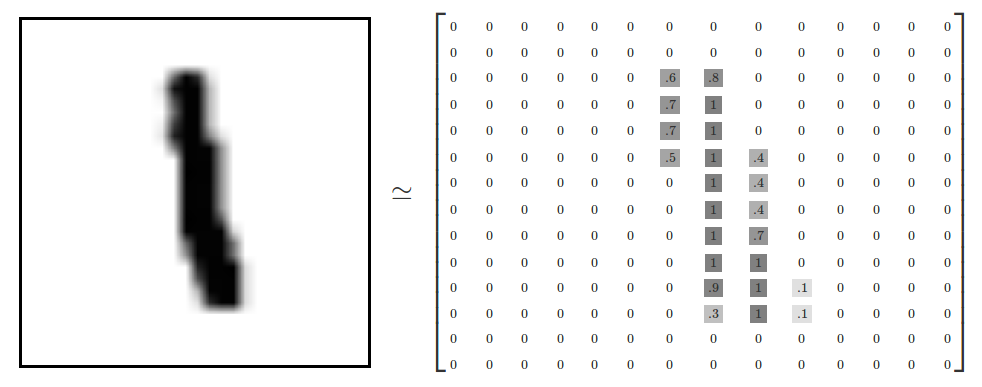
\includegraphics[width=0.9\textwidth]{figures/mnist-x.png}
\caption{MNIST样本数据表示}
 \label{fig:mnist-x}
\end{figure}

因此,在\ascii{MNIST}训练数据集中,\code{mnist.train.images}是一个\code{[60000, 784]}的二维矩阵。其中,矩阵中每一个元素,表示图片中某个像素的强度值,其值介于0和1之间。如\refig{mnist-train-xs}所示。

\begin{figure}[H]
\centering
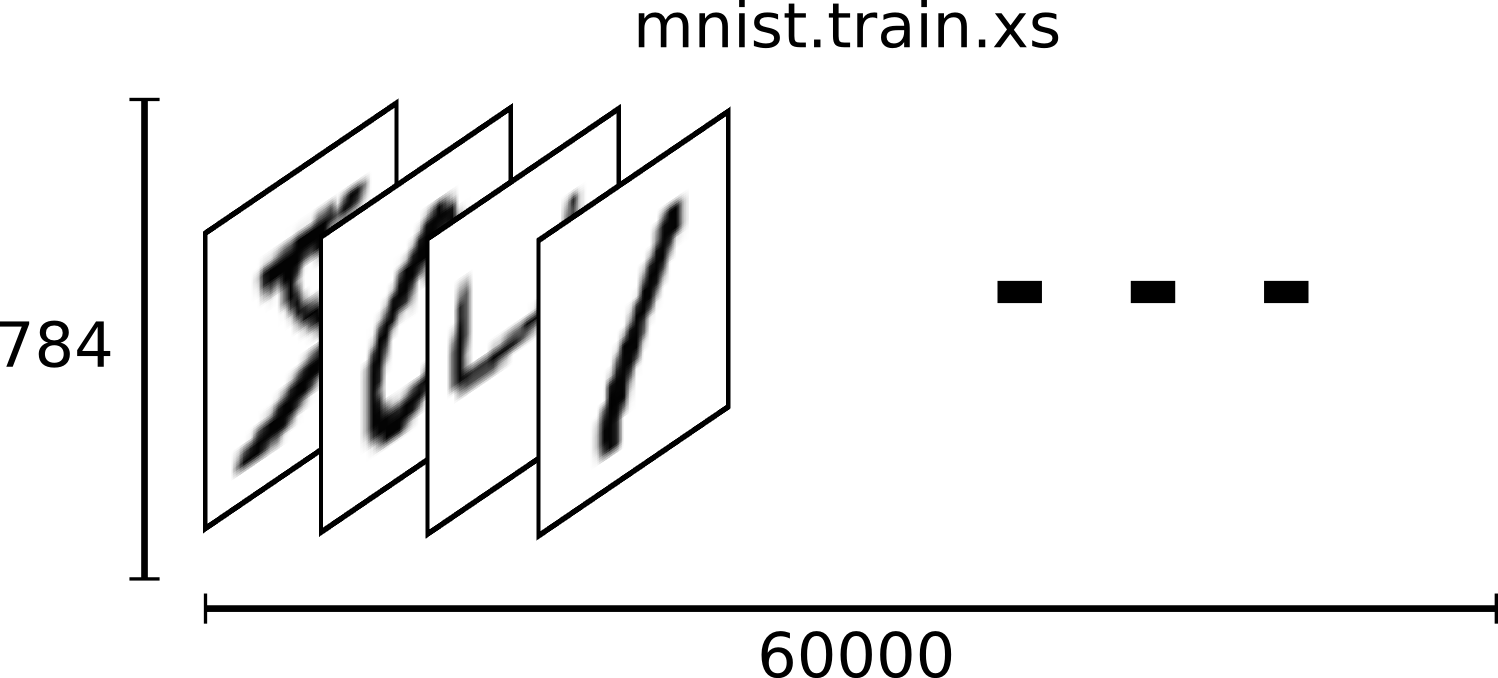
\includegraphics[width=0.9\textwidth]{figures/mnist-train-xs.png}
\caption{MNIST训练数据集:输入数据集}
 \label{fig:mnist-train-xs}
\end{figure}

相对应地,\ascii{MNIST}数据集的标签是介于\ascii{0}到\ascii{9}的数字。此处,样本的标签使用\ascii{\quo{one-hot}}的向量表示。因此,\code{mnist.train.labels}是一个\code{[60000, 10]}的二维矩阵。如\refig{mnist-train-ys}所示。

\begin{figure}[H]
\centering
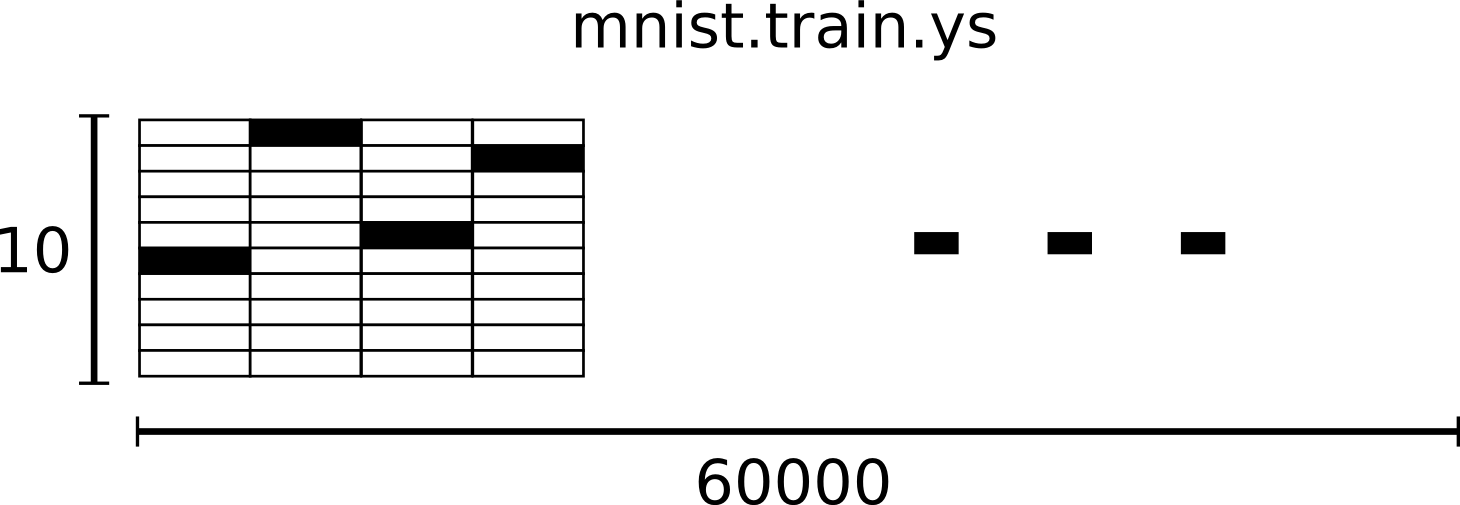
\includegraphics[width=0.9\textwidth]{figures/mnist-train-ys.png}
\caption{MNIST训练数据集:标签数据集}
 \label{fig:mnist-train-ys}
\end{figure}

\end{content}

\section{图示说明}

\begin{content}

为了更好地可视化整个训练过程,使用了\ascii{5}种面板。如\refig{mnist-training-digits}所示,表示\ascii{batch\_size}为\ascii{100}时,一个批次的训练样本。其中,白色背景表示数字被正确识别;而红色背景表示数字被误分类,手写数字的左侧标识正确的标签值,而右侧表示错误的预测值。

\ascii{MNIST}拥有\ascii{50000}个训练样本,如果\ascii{batch\_size}为\ascii{100},则需要迭代\ascii{500}次将完整地遍历一次训练样本的数据集,常称为一个\ascii{epoch}。

\begin{figure}[H]
\centering
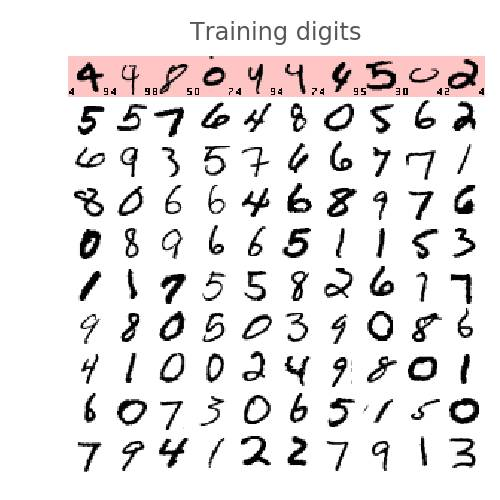
\includegraphics[width=0.6\textwidth]{figures/mnist-training-digits.jpeg}
\caption{一次mini-batch的训练样本数据集,其中batch\_size=100}
 \label{fig:mnist-training-digits}
\end{figure}

如\refig{mnist-test-digits}所示,\ascii{MNIST}使用了规模为\ascii{10000}的测试样本数据集测试模型的当前精度。其中,左侧表示目前模型的大致精度;同样地,白色背景表示数字被正确识别;而红色背景表示数字被误分类,手写数字的左侧标识正确的标签值,而右侧表示错误的预测值。

\begin{figure}[H]
\centering
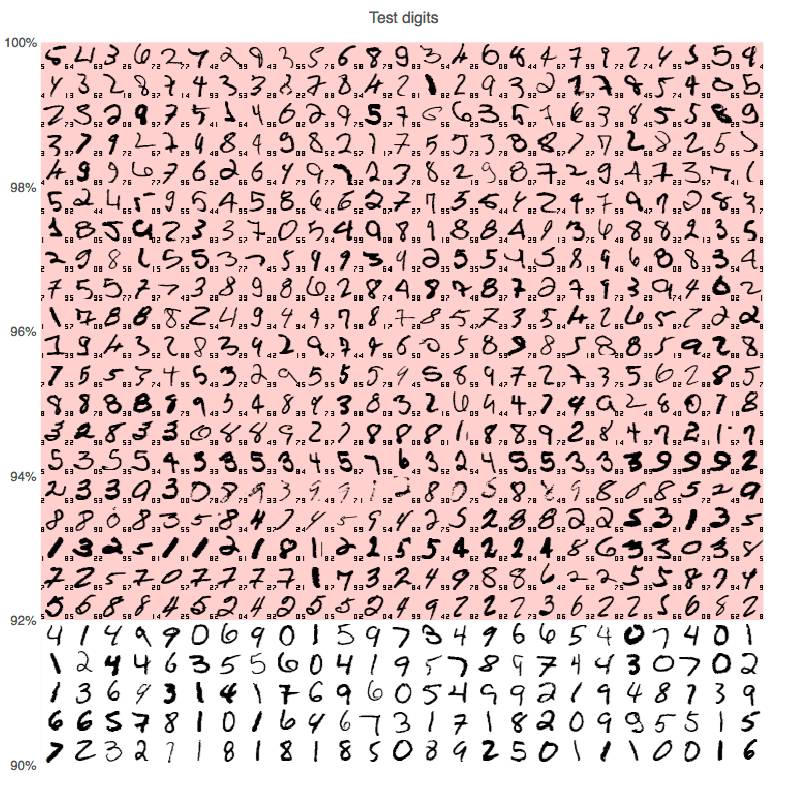
\includegraphics[width=0.6\textwidth]{figures/mnist-test-digits.jpeg}
\caption{当前的模型精度:基于测试样本数据集}
 \label{fig:mnist-test-digits}
\end{figure}

如\refig{mnist-cross-entropy-loss-fig}所示,使用交叉熵函数量化预测值与标签值之前的误差。其中,\ascii{x}轴表示迭代的次数,\ascii{y}轴表示损失值。

\begin{figure}[H]
\centering
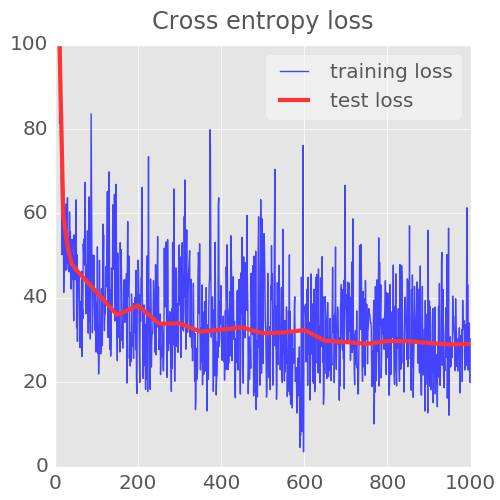
\includegraphics[width=0.6\textwidth]{figures/mnist-cross-entropy-loss-fig.jpeg}
\caption{训练和测试的交叉熵损失}
 \label{fig:mnist-cross-entropy-loss-fig}
\end{figure}

如\refig{mnist-accuracy-fig}所示,可以实时计算得到模型在当前训练数据集和测试集上的精度。其中,\ascii{x}轴表示迭代的次数,\ascii{y}轴表示精度值。

\begin{figure}[H]
\centering
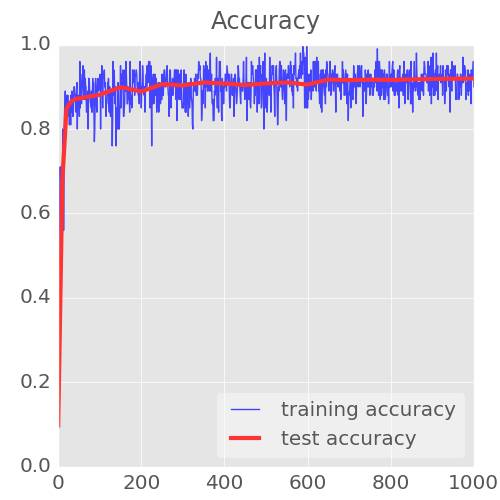
\includegraphics[width=0.6\textwidth]{figures/mnist-accuracy-fig.jpeg}
\caption{训练和测试的精度}
 \label{fig:mnist-accuracy-fig}
\end{figure}

如\refig{mnist-weight-fig.png}所示,对于模型的每一个训练参数(包括偏置),可以统计得到其对应的数值分布图。

\begin{figure}[H]
\centering
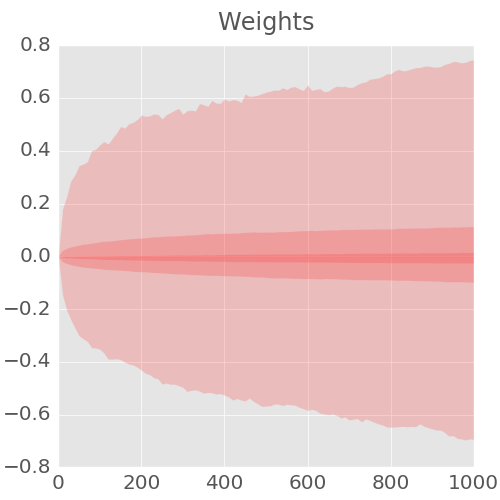
\includegraphics[width=0.6\textwidth]{figures/mnist-weight-fig.png}
\caption{权重分布图}
 \label{fig:mnist-weight-fig}
\end{figure}

\end{content}

\section{单层感知器}

\begin{content}

首先,尝试构建\ascii{10}个神经元的单层感知器。对于诸如手写数字识别的多分类问题,常常使用\ascii{softmax}的激活函数。

如\refig{mnist-slp}所示,对于任意一个输出神经元$n$,其线性加权和为$L_n$;然后,对$L_n$实施\ascii{softmax}的激活函数。


\begin{figure}[H]
\centering
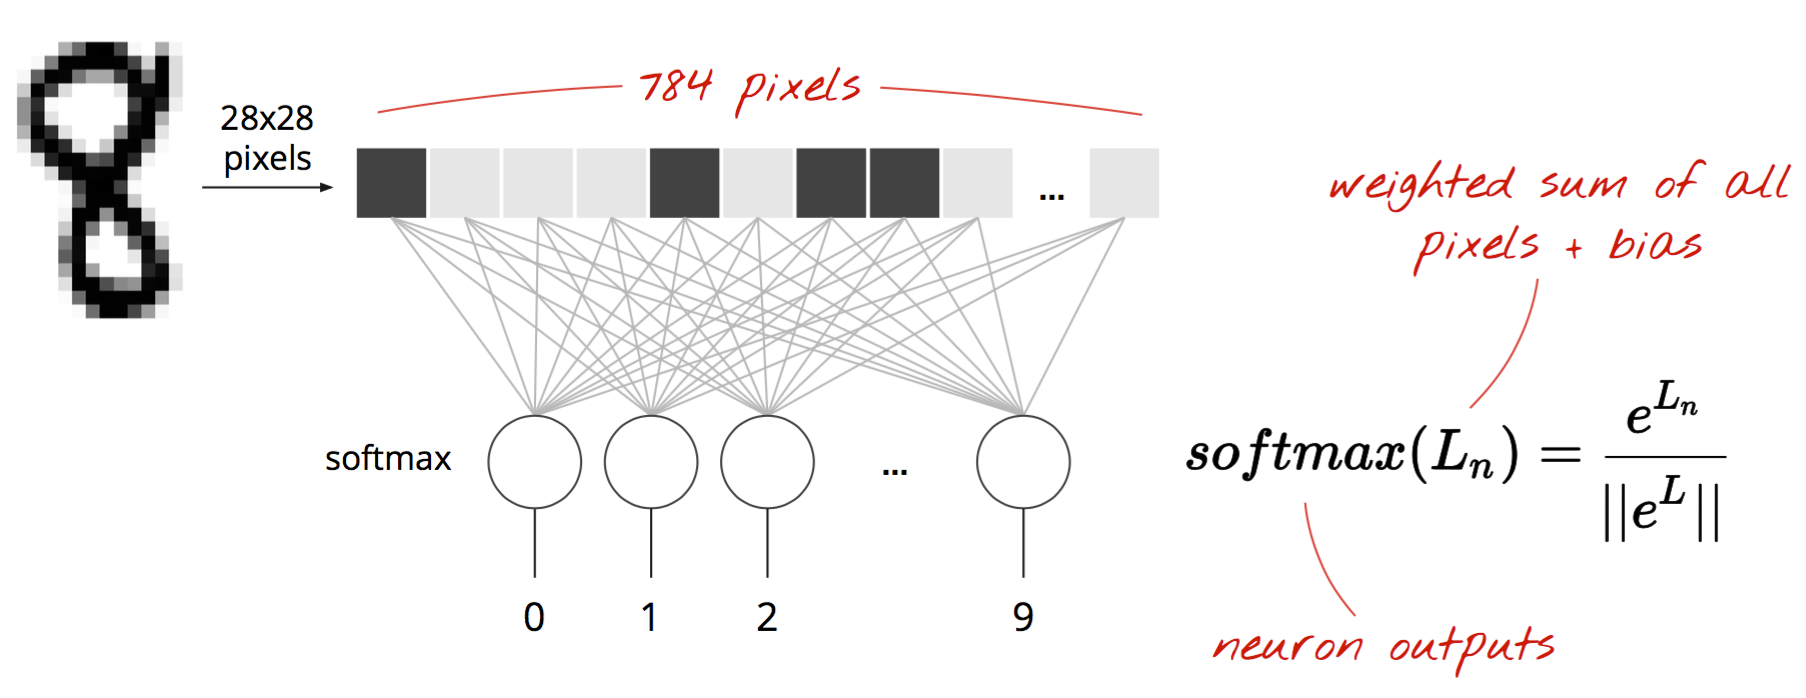
\includegraphics[width=0.8\textwidth]{figures/mnist-slp.png}
\caption{单层感知器}
 \label{fig:mnist-slp}
\end{figure}

\subsection{定义模型}

接下来,使用\tf{}完成该模型的搭建和训练。

\subsubsection{输入和标签}

首先,使用\code{tf.placeholder}分别定义一个\ascii{mini-batch}的训练样本数据集。其中,\code{tf.placeholder}定义了一个占位的\ascii{OP};\code{None}表示未确定的样本数目,此处表示\code{batch\_size}的大小;
\code{Session.run}时,将通过\code{feed\_dict}的字典提供一个\ascii{mini-batch}的样本数据集。

\begin{leftbar}
\begin{python}
x = tf.placeholder(tf.float32, [None, 784]) 
t = tf.placeholder(tf.float32, [None, 10])
\end{python}
\end{leftbar}

\subsubsection{定义变量}

然后,使用\code{tf.Variable}定义模型参数。定义训练参数时,必须指定参数的初始化值;训练参数将根据初始化值,自动推演数据的类型,及其维度。

此外,参数在使用之前,必须完成初始化。此处,\code{init\_op}将初始化所有全局的训练参数。

\begin{leftbar}
\begin{python}
w = tf.Variable(tf.zeros([784, 10]))
b = tf.Variable(tf.zeros([10]))

init_op = tf.global_variables_initializer()
\end{python}
\end{leftbar}

\subsubsection{模型定义}

接下来,便可以很容易地得到多分类问题的单层感知器模型。

\begin{leftbar}
\begin{python}
y = tf.nn.softmax(tf.matmul(x, w) + b)
\end{python}
\end{leftbar}

如\refig{mnist-linear-sum}所示,首先计算\code{x}与\code{w}的矩阵乘法,让后将\code{b}广播(\ascii{broadcast})到矩阵的每一行相加,最终得到训练参数的线性加权和。

\begin{figure}[H]
\centering
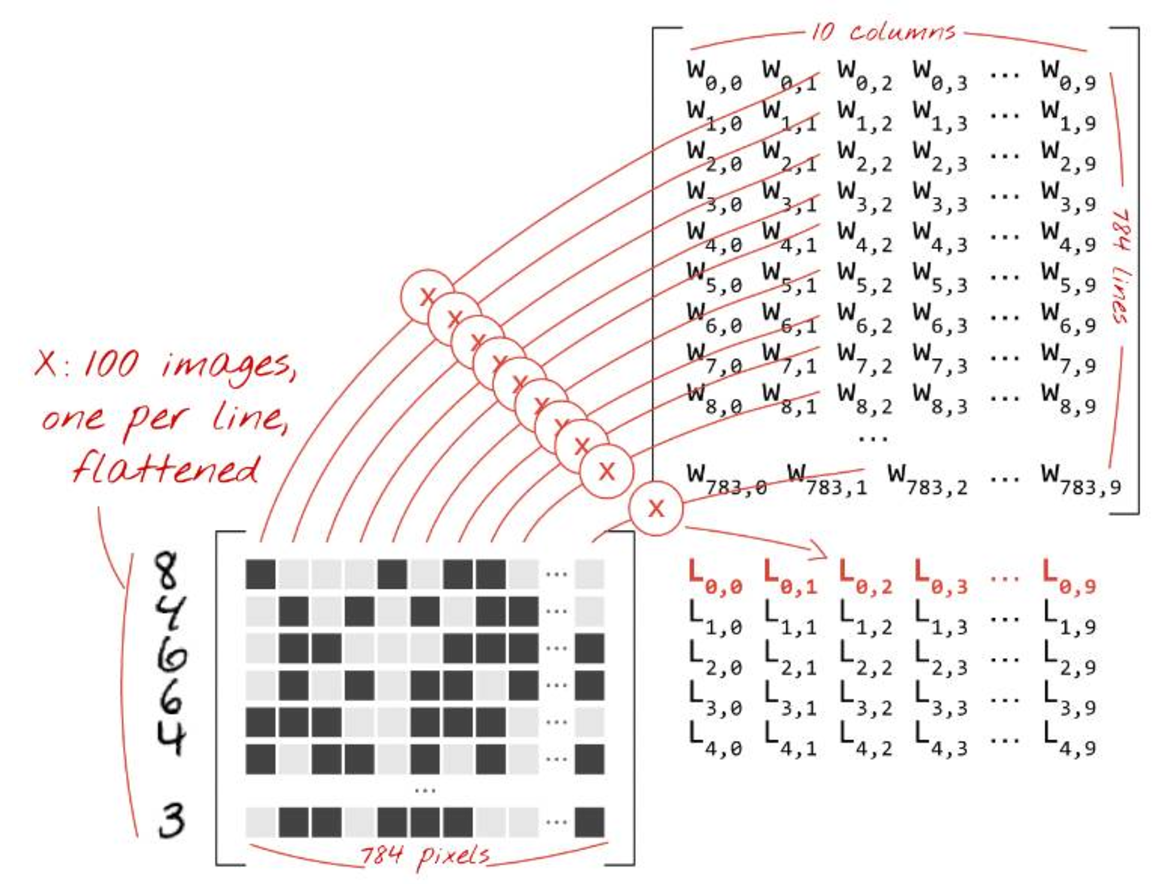
\includegraphics[width=0.8\textwidth]{figures/mnist-linear-sum.png}
\caption{线性和}
 \label{fig:mnist-linear-sum}
\end{figure}

如\refig{mnist-softmax}所示,\ascii{softmax}将逐行实施运算,最终,\code{y}的大小为\code{[100, 10]}。

\begin{figure}[H]
\centering
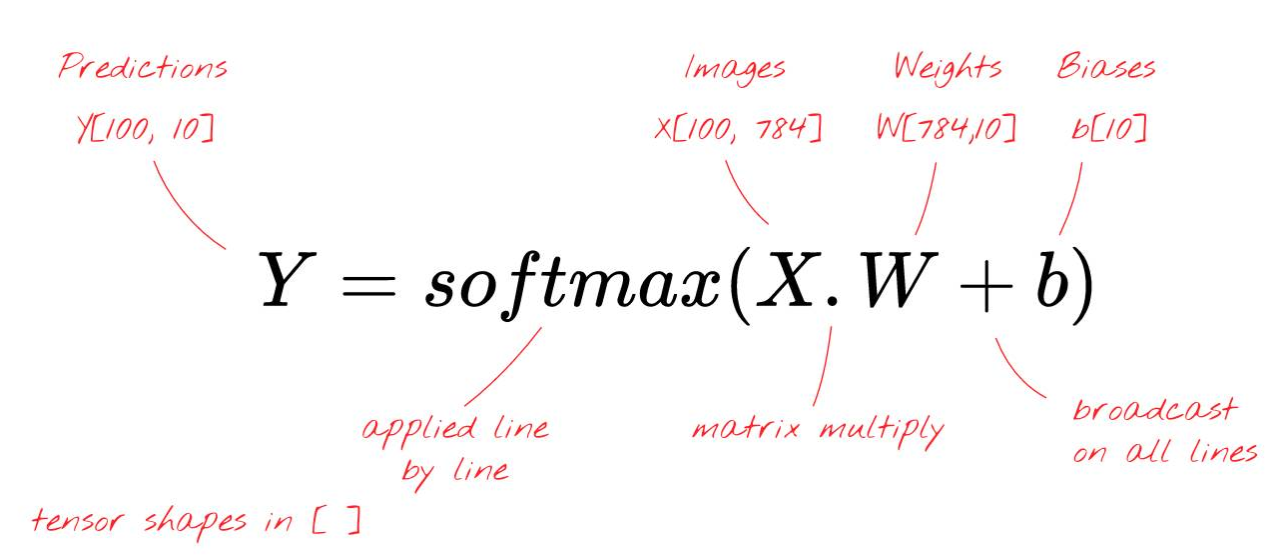
\includegraphics[width=0.8\textwidth]{figures/mnist-softmax.png}
\caption{激活函数:softmax}
 \label{fig:mnist-softmax}
\end{figure}

\subsubsection{损失函数}

对于多分类问题,可以使用交叉熵的损失函数。

\begin{leftbar}
\begin{python}
cross_entropy = -tf.reduce_sum(t * tf.log(y))
\end{python}
\end{leftbar}

如\refig{mnist-cross-entropy}所示,\code{t}和\code{y}的大小都为\code{[100, 10]};特殊地,\code{t}的每一行都是一个\quo{\ascii{one-hot}}向量。

对\code{y}实施\code{tf.log}操作,也将得到一个大小为\code{[100, 10]}的矩阵。最终,\code{tf.reduce\_sum}将矩阵中所有元素相加,得到一个标量(\ascii{scalar})值。

\begin{figure}[H]
\centering
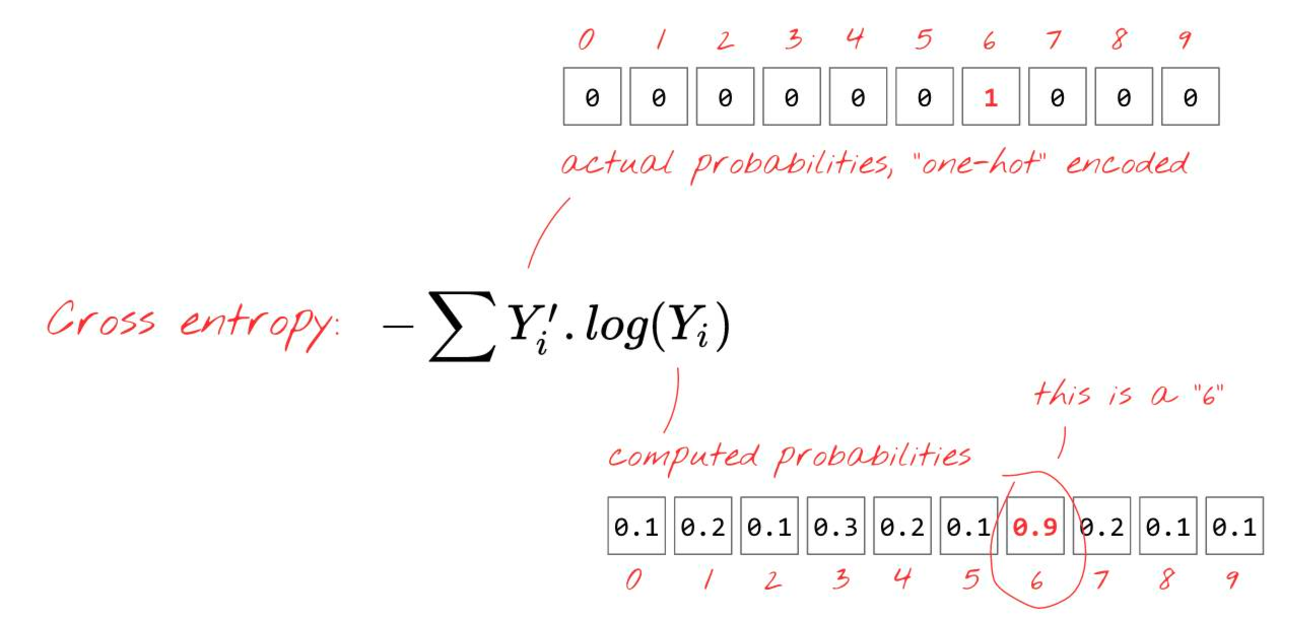
\includegraphics[width=0.8\textwidth]{figures/mnist-cross-entropy.png}
\caption{交叉熵损失函数}
 \label{fig:mnist-cross-entropy}
\end{figure}

\subsubsection{精度}

\code{tf.argmax(y,1)}将按第\ascii{1}个维度计算最大值的索引。既按照${{\text{y}}_{{\text{100}} \times {\text{10}}}}$的每一行,计算得到在每一行中最大值的的索引值。因此,\code{tf.argmax(y,1)}将得到大小为\code{[100, 1]}的矩阵,或大小为\ascii{100}的向量。同样地,\code{tf.argmax(t,1)}也是一个大小为\ascii{100}的向量。

然后,使用\code{tf.equal}将它们逐元素(\ascii{element-wise})进行相等性比较,得到大小为\ascii{100}的布尔向量。为了计算精度,先将布尔向量转别为数值向量,最终求取该数值向量的均值。

\begin{leftbar}
\begin{python}
is_correct = tf.equal(tf.argmax(y,1), tf.argmax(t,1))
accuracy = tf.reduce_mean(tf.cast(is_correct, tf.float32))
\end{python}
\end{leftbar}

\subsection{优化算法}

接下来,使用梯度下降算法实现交叉熵损失函数的最小化。其中,\code{learning\_rate}表示学习速率,描述参数更新的快慢和步伐大小,是一个典型的超参。如\refig{mnist-gd}所示。

\begin{leftbar}
\begin{python}
optimizer = tf.train.GradientDescentOptimizer(learning_rate=0.003)
train_step = optimizer.minimize(cross_entropy)
\end{python}
\end{leftbar}

\begin{figure}[H]
\centering
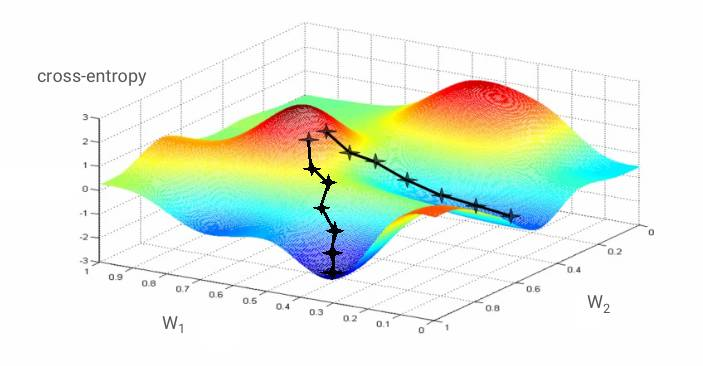
\includegraphics[width=0.8\textwidth]{figures/mnist-gd.jpeg}
\caption{梯度下降算法}
 \label{fig:mnist-gd}
\end{figure}

\subsection{训练模型}

在此之前,\tf{}仅构造计算图,并没有启动计算图的执行。接下来,客户端创建一个会话,建立与本地或远端计算设备集的通道,启动计算图的执行过程。

首先,完成训练参数的初始化。通过运行模型参数的初始化子图,并发地执行各个训练参数的初始化器,将初始值就地修改到相应的训练参数内。

\begin{leftbar}
\begin{python}
with tf.Session() as sess:
  sess.run(init_op)
\end{python}
\end{leftbar}

然后,开始迭代地执行\code{train\_op},完成模型的训练。其中,每\ascii{100}次迭代,计算当前模型在训练数据集及测试数据集的精度和损失。

\begin{leftbar}
\begin{python}
with tf.Session() as sess:
  for step in range(1000):
    batch_xs, batch_ys = mnist.train.next_batch(100)        
    sess.run(train_step, feed_dict={x: batch_xs, t: batch_ys})
    
    if step % 100 == 0:
      acc, loss = sess.run([accuracy, cross_entropy], 
        feed_dict={x: batch_xs, t: batch_ys})

      acc, loss = sess.run([accuracy, cross_entropy], 
        feed_dict={x: mnist.test.images, t: mnist.test.labels}) 
\end{python}
\end{leftbar}

通过\ascii{1000}次迭代,可得到大约\percent{92}的精度。

\begin{figure}[H]
\centering
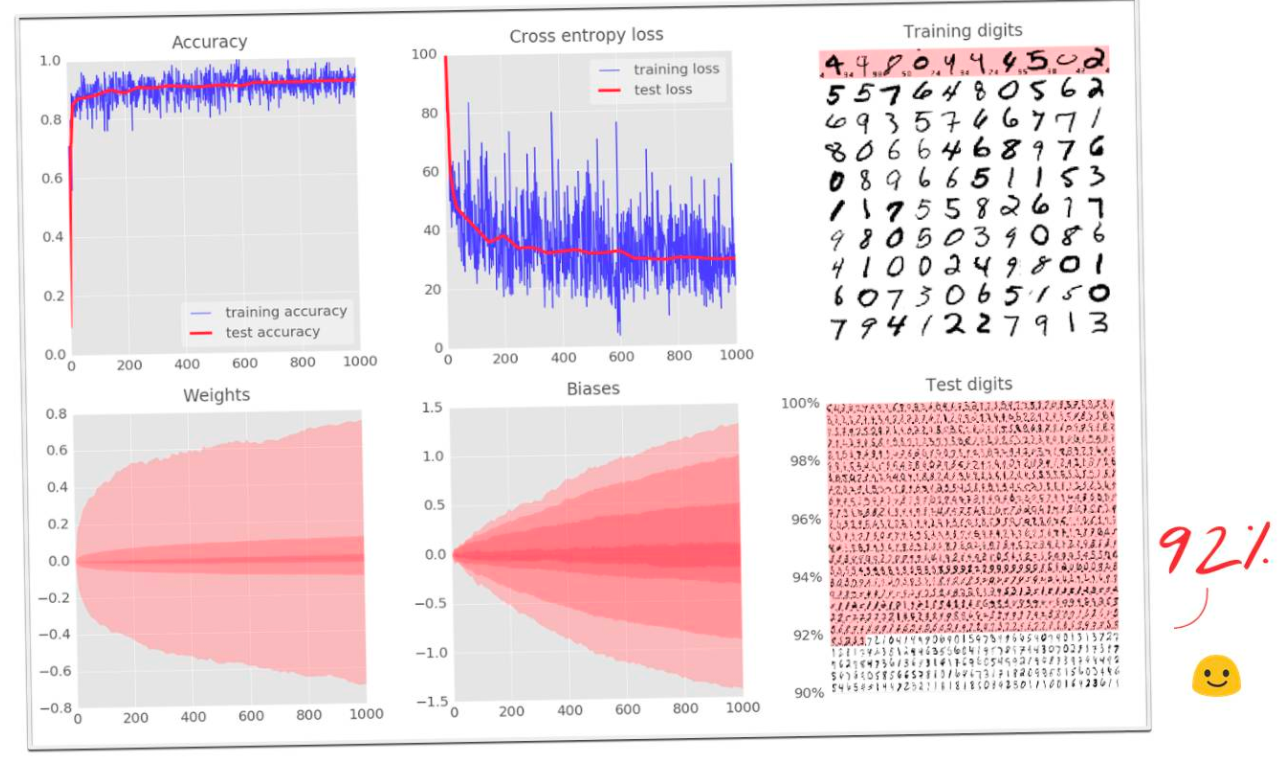
\includegraphics[width=0.8\textwidth]{figures/mnist-slp-accuracy.png}
\caption{可视化:单层感知器,运行1000次step}
 \label{fig:mnist-slp-accuracy}
\end{figure}

\end{content}

\section{多层感知器}

\begin{content}

为了进一步提高精度,接下来尝试搭建\ascii{5}层的多层感知器模型。

\begin{figure}[H]
\centering
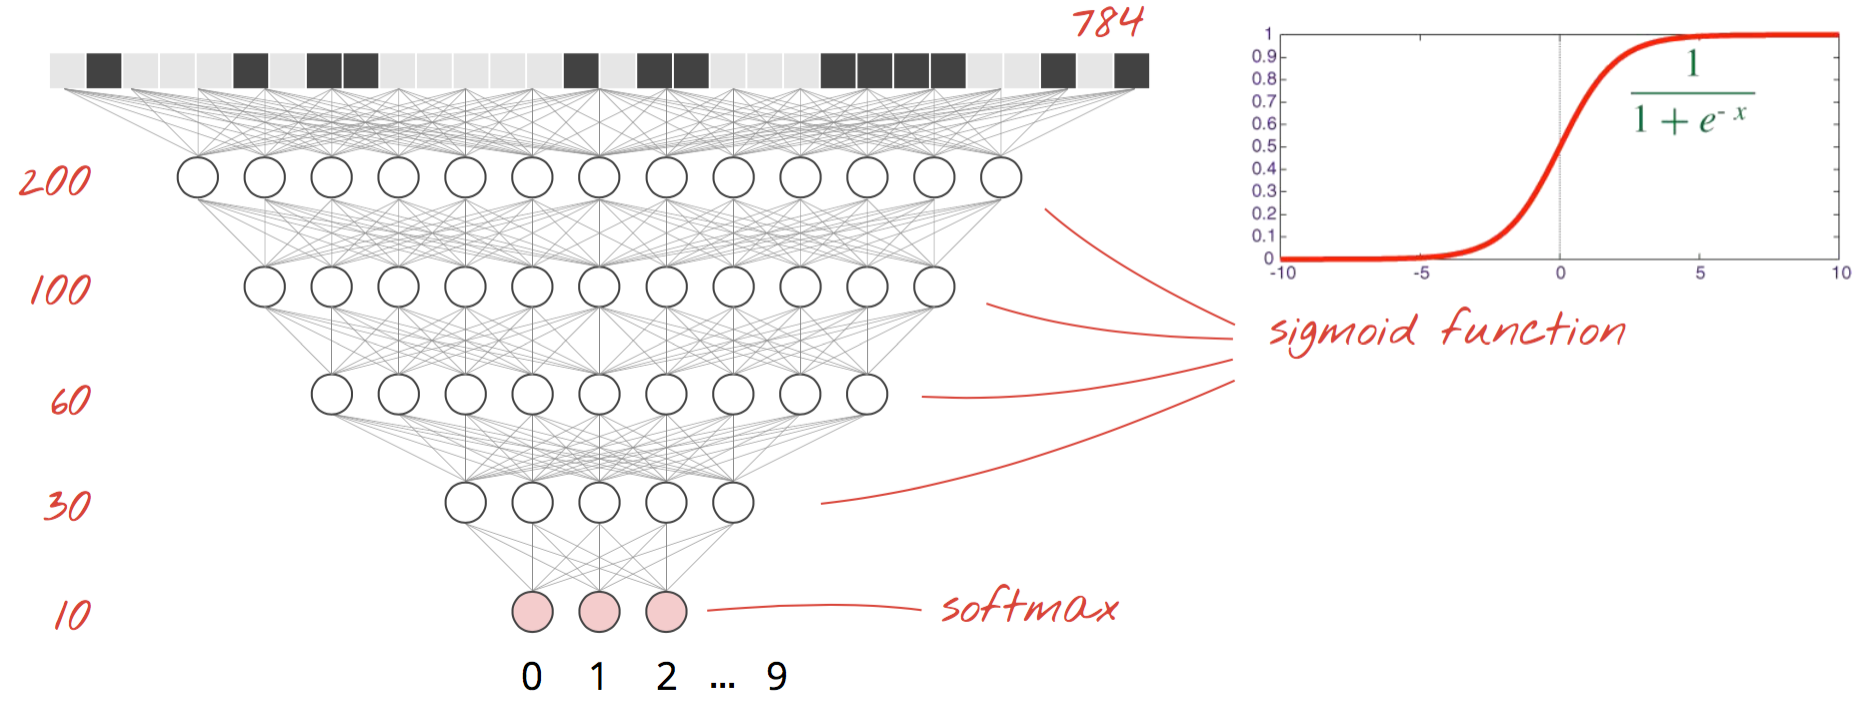
\includegraphics[width=0.8\textwidth]{figures/mnist-5-layer.png}
\caption{5层感知器}
 \label{fig:mnist-5-layer}
\end{figure}

\subsection{定义模型}

相对于上一节中尝试的单层感知器,此处定义每一个隐式层的权重时,并没有使用常量表示的初始值,而使用满足某种数据分布特征的随机值。

\begin{leftbar}
\begin{python}
K = 200
L = 100
M = 60
N = 30

w1 = tf.Variable(tf.truncated_normal([28*28, K] ,stddev=0.1)) 
b1 = tf.Variable(tf.zeros([K]))

w2 = tf.Variable(tf.truncated_normal([K, L], stddev=0.1))
b2 = tf.Variable(tf.zeros([L]))

w3 = tf.Variable(tf.truncated_normal([L, M], stddev=0.1)) 
b3 = tf.Variable(tf.zeros([M]))

w4 = tf.Variable(tf.truncated_normal([M, N], stddev=0.1)) 
b4 = tf.Variable(tf.zeros([N]))

w5 = tf.Variable(tf.truncated_normal([N, 10], stddev=0.1)) 
b5 = tf.Variable(tf.zeros([10]))
\end{python}
\end{leftbar}

在定义每一个隐式层时,采用\ascii{sigmoid}的激活函数。最最后的输出层,采用\ascii{softmax}的激活函数。

\begin{leftbar}
\begin{python}
y1 = tf.nn.sigmoid(tf.matmul(x,  w1) + b1)
y2 = tf.nn.sigmoid(tf.matmul(y1, w2) + b2)
y3 = tf.nn.sigmoid(tf.matmul(y2, w3) + b3)
y4 = tf.nn.sigmoid(tf.matmul(y3, w4) + b4)
y  = tf.nn.softmax(tf.matmul(y4, w5) + b5)
\end{python}
\end{leftbar}

\subsection{训练模型}

\end{content}

\section{优化技术}

\begin{content}

\subsection{激活函数:RELU}

在深度模型中,不适合使用\ascii{sigmoid}激活函数。它将把所有的值都挤到了\ascii{0}到\ascii{1}之间;随着网络层次的增加,导致梯度消失。

\begin{figure}[H]
\centering
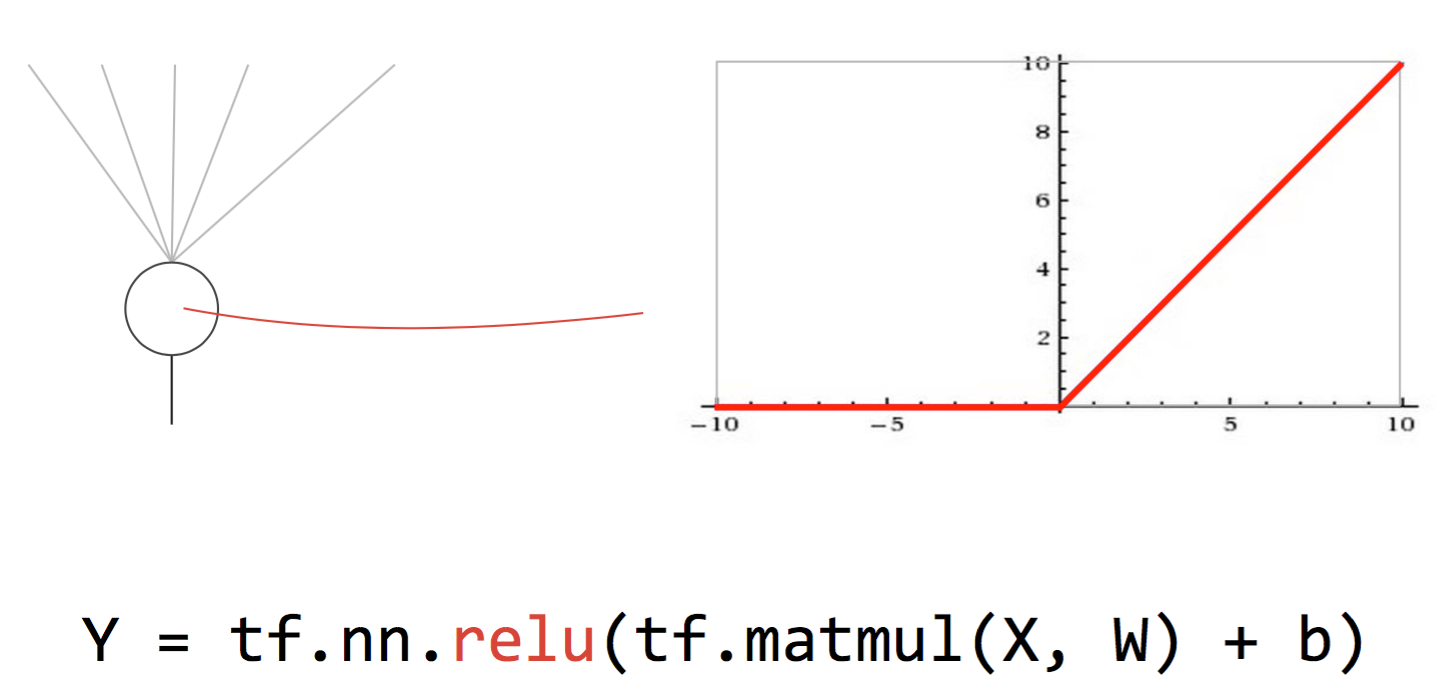
\includegraphics[width=0.8\textwidth]{figures/mnist-relu.png}
\caption{ReLU激活函数}
 \label{fig:mnist-relu}
\end{figure}

可以使用\ascii{ReLU}激活函数,不仅避免了\ascii{sigmoid}导致的一些问题,而且能够加快更快的初始的收敛速度。如\refig{mnist-sigmoid-to-relu}所示,前300次迭代,使用\ascii{ReLU}相对于使用\ascii{sigmoid},其初始收敛速度提升显著。

\begin{figure}[H]
\centering
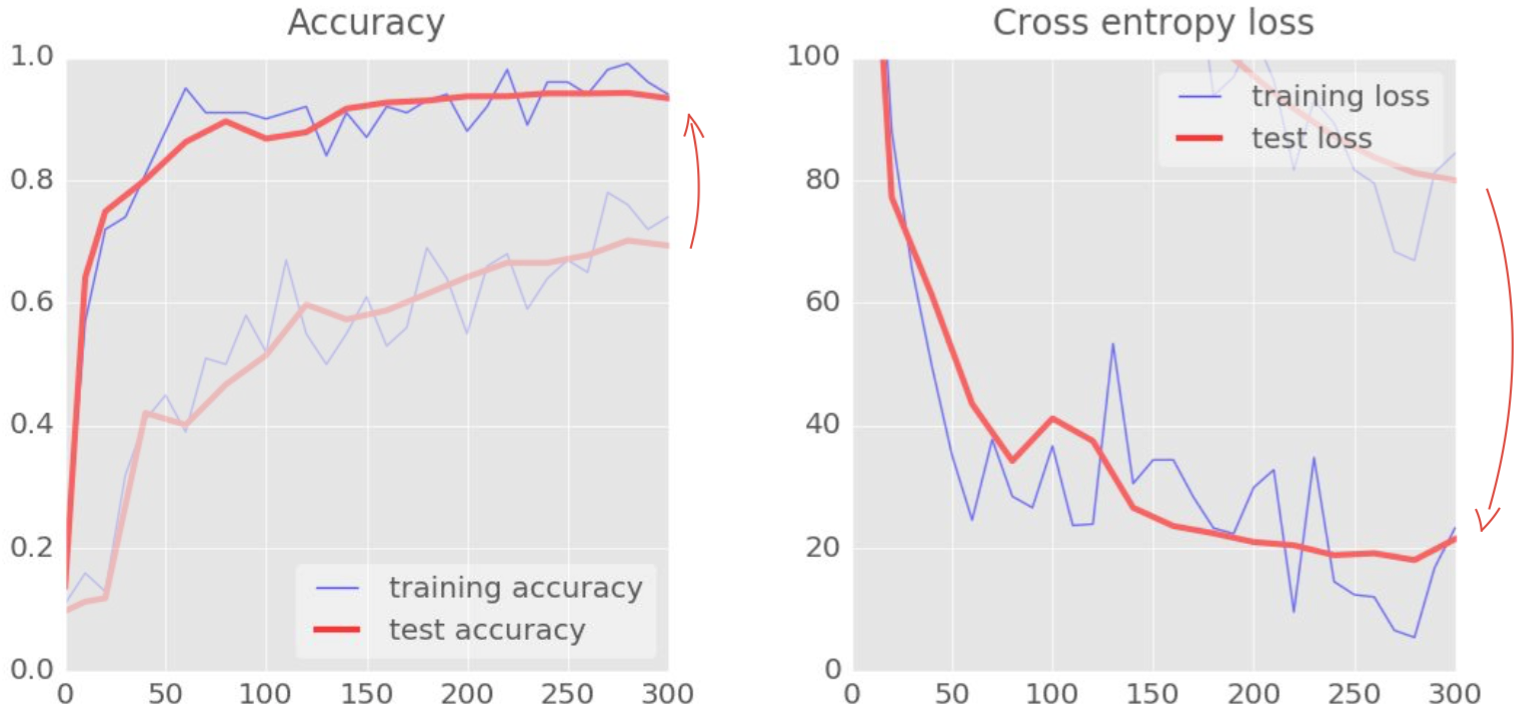
\includegraphics[width=0.8\textwidth]{figures/mnist-sigmoid-to-relu.png}
\caption{应用ReLU激活函数:初始收敛速度提升显著}
 \label{fig:mnist-sigmoid-to-relu}
\end{figure}

\subsection{学习速率衰减}

随着网路层次的增加,及其应用相关优化技术后,模型的精度能够得到\percent{98}左右,但很难得到一个稳定的精度。如\refig{mnist-lr-too-larger}所示,精度和损失抖动相当明显。

\begin{figure}[H]
\centering
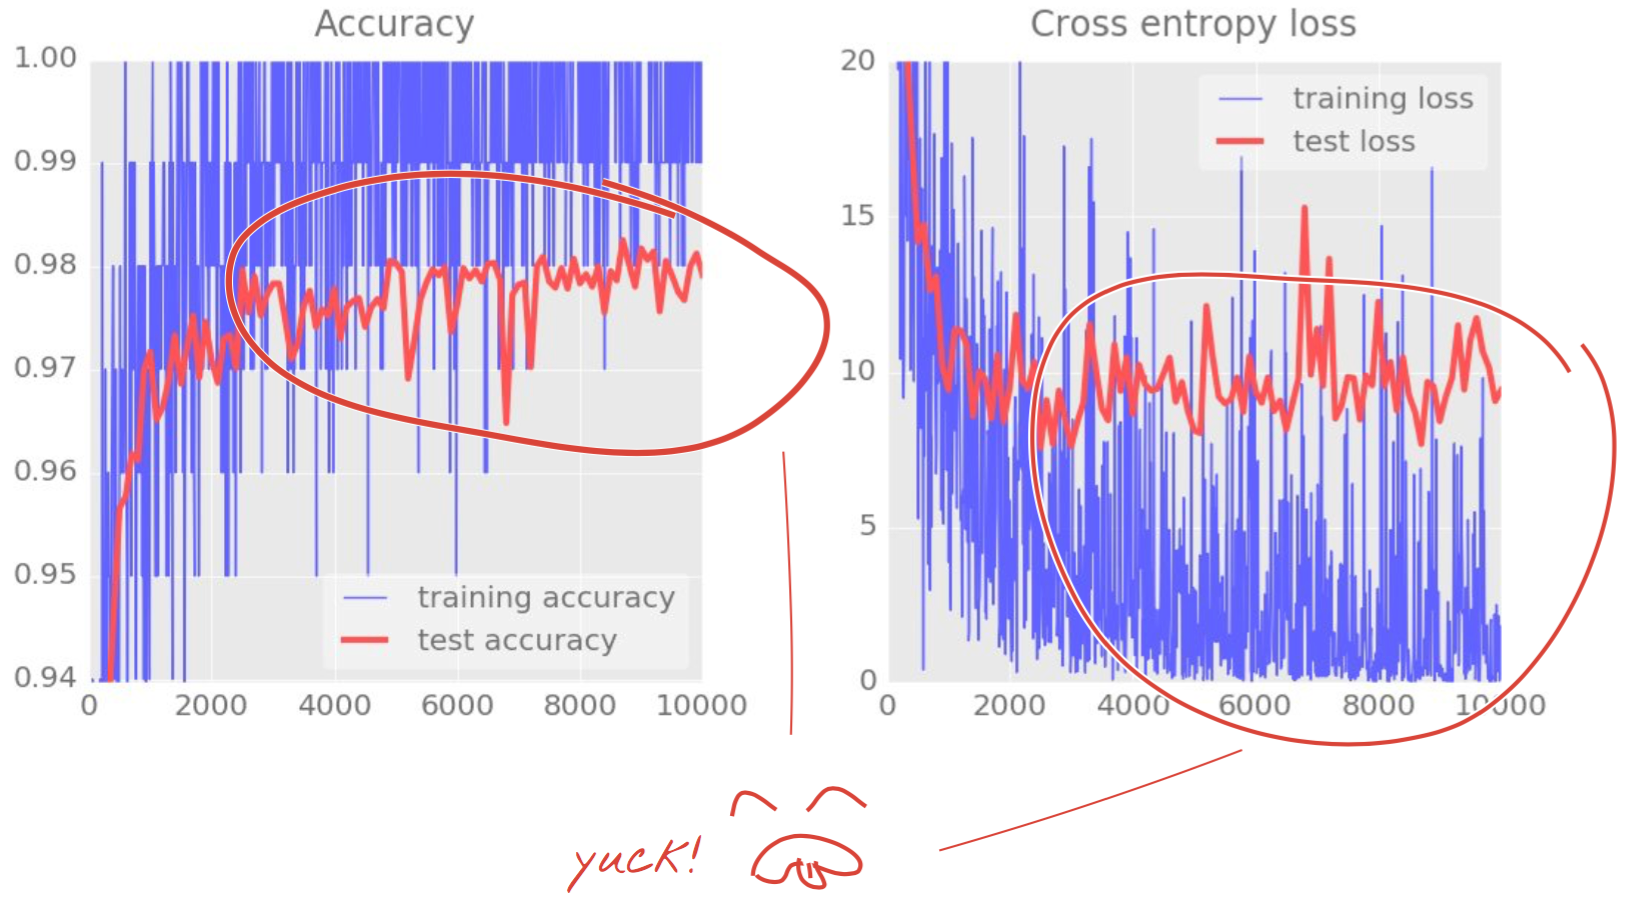
\includegraphics[width=0.8\textwidth]{figures/mnist-lr-too-larger.png}
\caption{噪声抖动:学习速率过大}
 \label{fig:mnist-lr-too-larger}
\end{figure}

可以采用更好的优化算法,例如\code{AdamOptimizer},随着迭代过程的次数,学习速率指数衰减,可以得到一个更稳定的精度。如\refig{mnist-apply-learning-rate-decay}所示。

\begin{figure}[H]
\centering
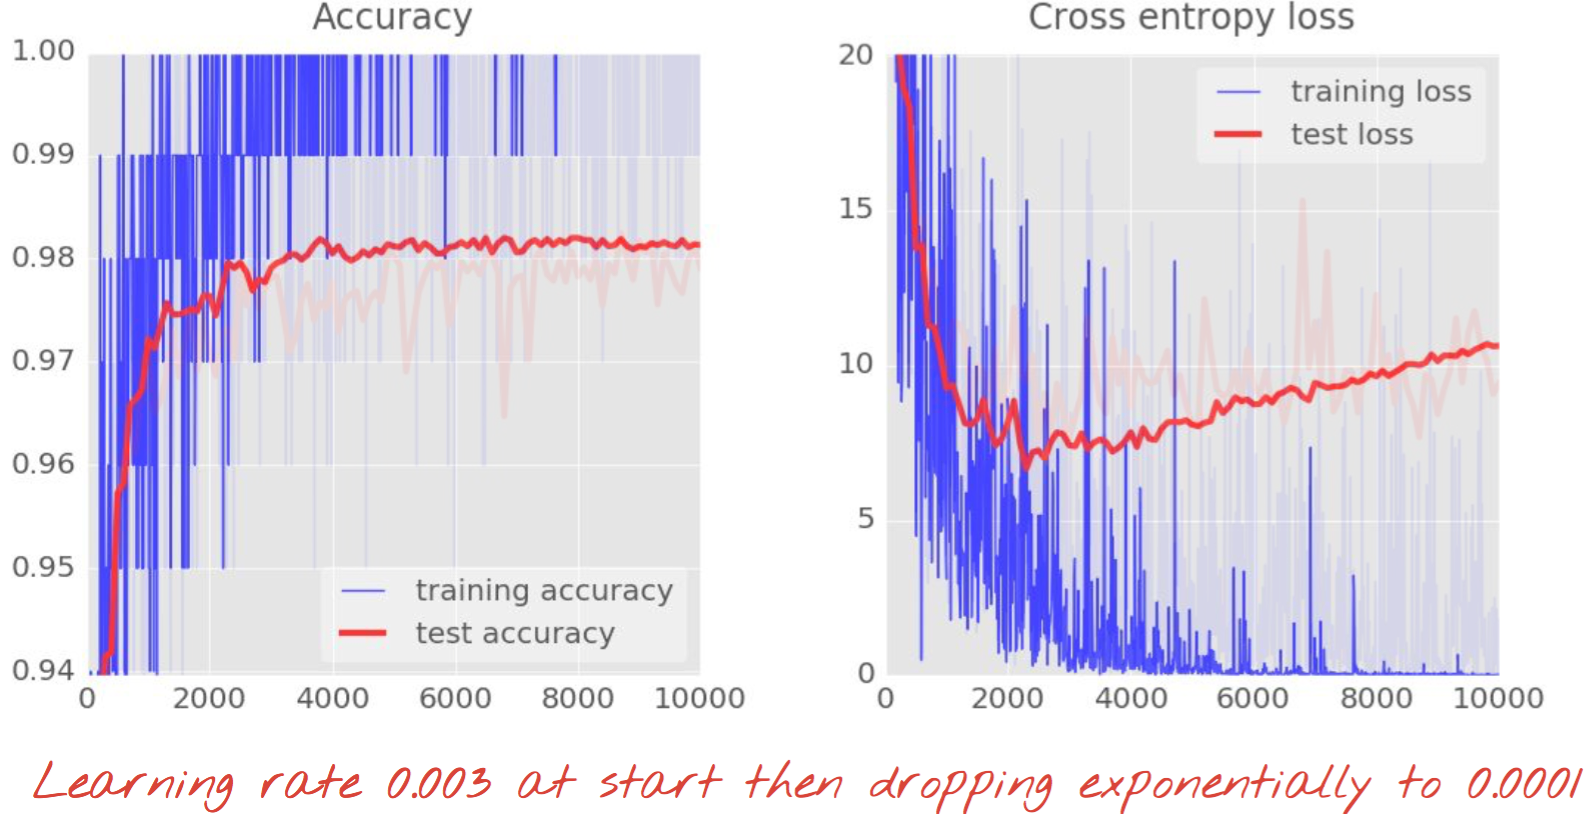
\includegraphics[width=0.8\textwidth]{figures/mnist-apply-learning-rate-decay.png}
\caption{应用Adam优化算法后,精度趋于稳定}
 \label{fig:mnist-apply-learning-rate-decay.png}
\end{figure}

\subsection{应用Dropout}

但是,训练集与测试集上的损失曲线出现分离,出现明显的过拟合现象。

\begin{figure}[H]
\centering
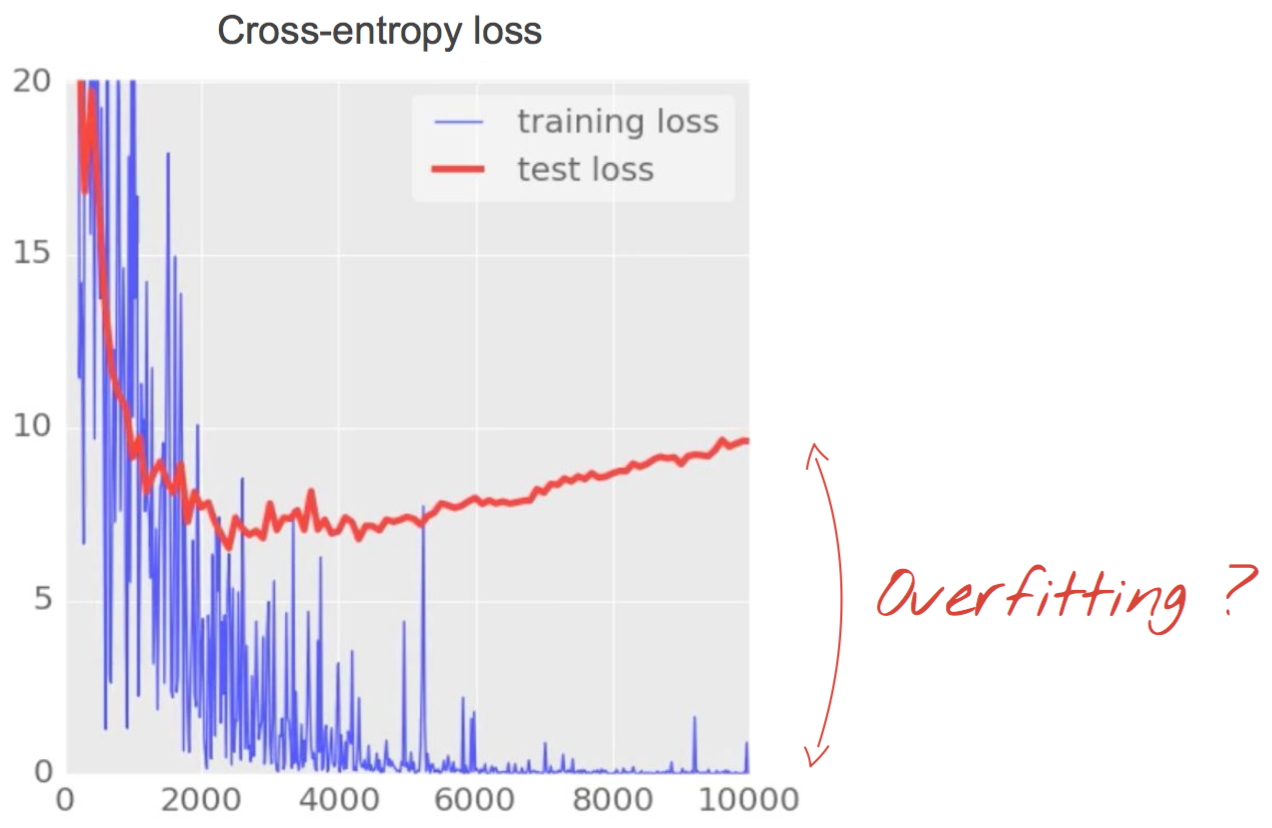
\includegraphics[width=0.8\textwidth]{figures/mnist-overfitting.png}
\caption{过拟合}
 \label{fig:mnist-overfitting}
\end{figure}

如\refig{mnist-dropout}所示,可以在训练时,对每一层的输出实施\ascii{dropout}操作,而在推理时丢弃\ascii{dropout},减低过拟合的问题。

\begin{figure}[H]
\centering
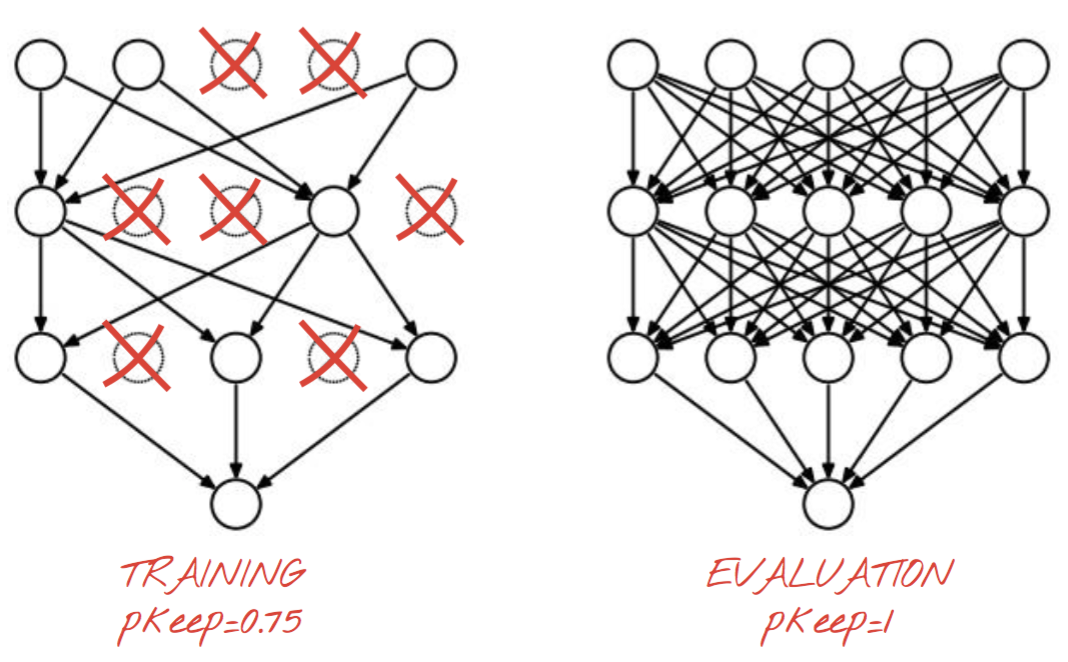
\includegraphics[width=0.8\textwidth]{figures/mnist-dropout.png}
\caption{Dropout方法}
 \label{fig:mnist-dropout}
\end{figure}


\begin{figure}[H]
\centering
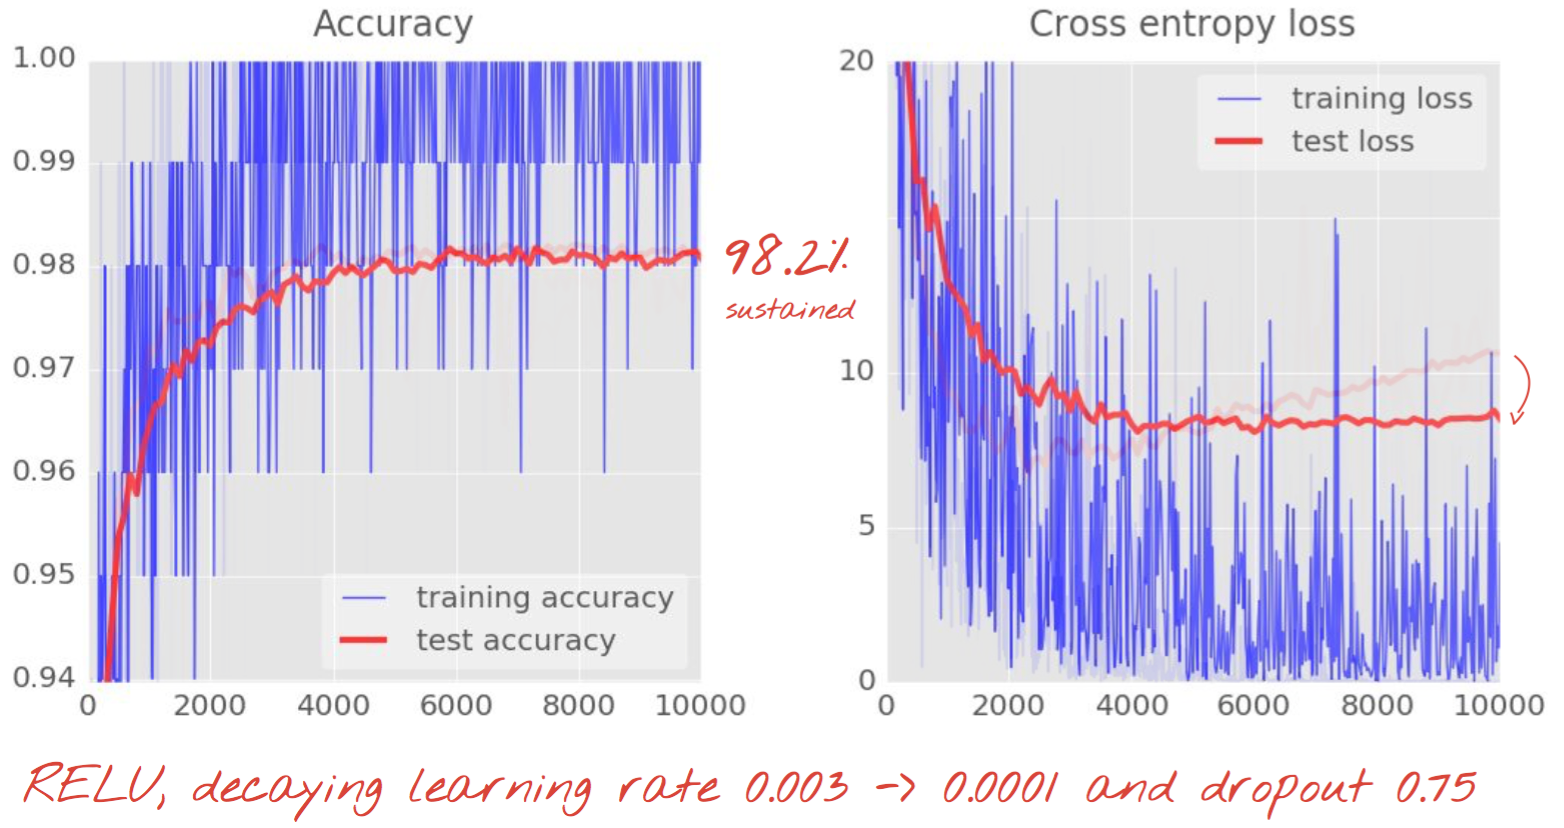
\includegraphics[width=0.8\textwidth]{figures/mnist-apply-dropout-result.png}
\caption{实施Dropout后,训练集与测试集的损失曲线再次重合}
 \label{fig:mnist-apply-dropout-result}
\end{figure}

\subsection{过拟合}

\end{content}
